% !TEX root = ../main.tex
\chapter{基于成对监督的细粒度跨模态图像检索}
行人重识别 (Person Re-identification, Person ReID) 旨在给定一个检索的行人图片, 在一个包含多个不同监控摄像头拍摄的不同的行人的图片数据库中检索出对应的行人图片。在所有的与 ReID 相关的研究中, 跨模态行人重识别 (Visible-to-thermal Person Re-identification, VT-REID) 在现阶段获得了研究人员的广泛关注。由于模态鸿沟 (Modality Gap), 跨模态变化 (Cross Modality Variation) 以及模态内变化 (Intra Modality Variation) 的存在, 跨模态行人重识别与传统行人重识别相比而言更加有挑战性。当前的算法一般通过两个分开的卷积神经网络 (Convolutional Neural Network, CNN) 将两个不同模态的图片映射到同一个特征空间, 然后通过各种铰链损失函数来进行度量学习。然而, 这种基于简单的CNN的网络很难捕捉到有判别性的模态恒定 (Modality Invariant)的特征, 从而导致了后续识别时的性能损失。本章提出了一个新型的学习模态恒定以及外表恒定 (Appearance Invariant)特征的框架网络, 以及一系列基于最大似然估计的损失函数来进行跨模态识别任务。本章提出的算法在跨模态识别的标准数据集 \textbf{RegDB} 和 \textbf{SYSU-MM01}上取得了先进的性能, 证明了算法的有效性以及先进性。
\section{引言}
智能安防是新时代智慧城市建设中不可缺少的一环。通过城市中各处不同型号不同分辨率的视频监控设备24小时的监控摄影, 现代城市生活的安全系数得到了极大的提高。其中的一个支撑智能安防的关键研究方向就是行人重识别。 行人重识别是通过在一个包含不同监控摄像头在不同视角拍摄的大量行人图片的数据库中精确的查找检索出给定的一个特定行人的照片~\cite{wang2016scale,zheng2017sift}。大部分现有的算法主要关注单模态可见光图像的检索 (Visible Images), 即检索的图片和数据库中的图像都是 RGB 图~\cite{ahmed2015improved,koestinger2012large, li2014deepreid, li2015multi, li2013learning, liao2015person, wu2016enhanced, xiao2016learning, zhu2017part, chen2017multi, ge2018fd, li2018harmonious,chen2021harmonious, tang2022harmonious, xu2018attention, yao2019deep, zheng2019joint}。\par
在现实生活中, 很大部分的犯罪行为发生在夜间低照明度的环境中, 传统的可见光摄像头无法捕捉到行人的有区别性的特征信息。因此, 现在的监控摄像头一般具有两种模式: 可见光模式和红外线模式。在光照充足的条件下, 监控摄像头会自动切换到可见光模式, 而当光照不足时, 会自动切换到红外线摄像模式。这样的场景催生了一个新的研究方向叫跨模态行人重识别, 并且获得了学术界和工业界的广泛关注~\cite{zheng2019joint}。
\begin{figure}[!htp]
    \centering
    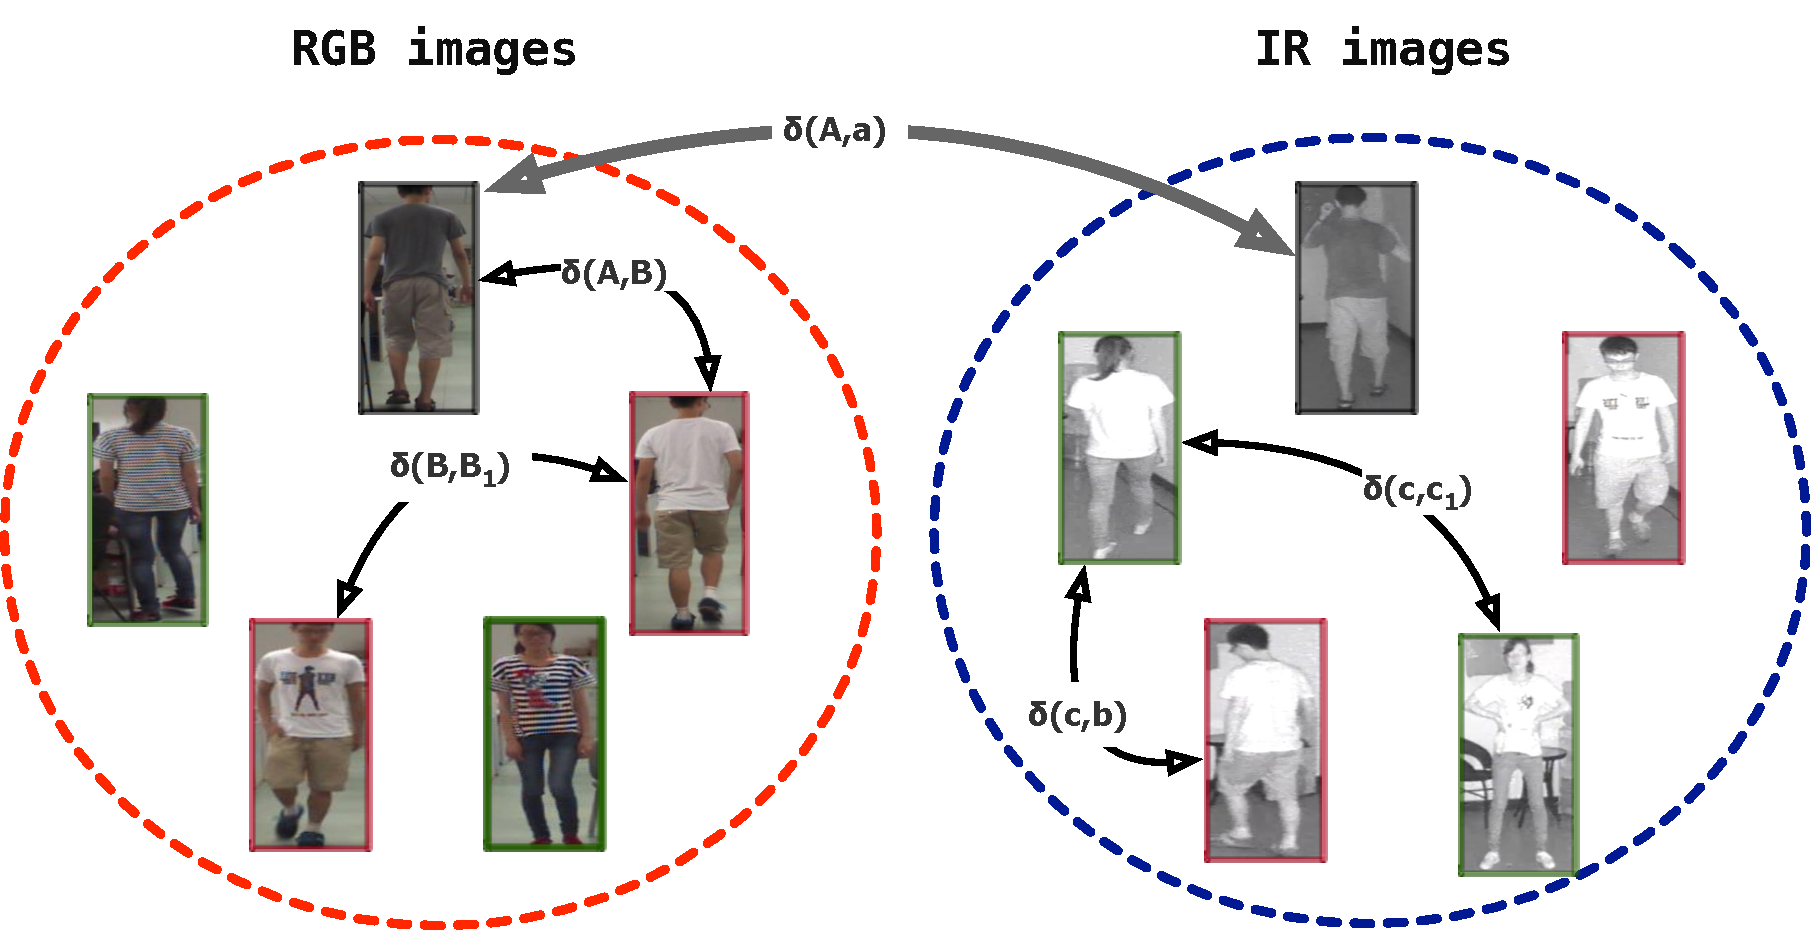
\includegraphics[width=14.5cm]{02/arch1.pdf} \\
    \bicaption[跨模态行人重识别介绍图]
      {跨模态行人重识别难点示意图, 图中展示出来跨模态的变化以及模态内的变化带来的难点。每一张被同色方框围住的图片属于同一个行人。由于模态的差异性以及变化带来的影响, 同一行人的距离 $\delta(A, a)$比不同行人的距离$\delta(A, B)$还大。 同时, 由于模态内的变化存在, 同一行人不同照片的距离 $\delta(c, c_1)$ 也超过了不同行人照片的距离$\delta(c, b)$。}
      {Illustration of the difficulty of VT-REID resulted from the modality discrepancy, cross-modality variation and intra-modality variation. Boxes with the same color denote pictures from the same person. Owing to the crossmodality discrepancy and variation, the intra-person distance$ \delta(A,a)$ is larger than the inter-person distance $\delta(A, B)$. Further, as demonstrated in the right part of the picture, intra-person distance $\delta(c,c_1)$ is larger than $\delta(c,b)$ caused by intra-modality variation.}
   \label{fig:arch1}
\end{figure} 
和传统行人重识别相比, VT-ReID 由于跨模态差异 (Cross-modality Discrepancy)的存在而尤其地具有挑战性, 如图~\ref{fig:arch1}。跨模态的差异一般是由于可见光和热度图成像使用的不同的光谱造成。同时, 如图~\ref{fig:arch1}所示, 由于捕捉行人图像的摄像机角度的差别, 以及行人外表着装等的改变带来的模态内的变化更加剧了跨模态检索的难度。\par
现阶段的跨模态行人重识别方法一般包含两个通用的流程: (1) ``\textbf{特征提取}'' 和 (2)``\textbf{相似度学习}'' 。对于``\textbf{特征提取}'', 现有的算法框架基本基于卷积神经网络例如 AlexNet 或者 ResNet 等来提取特征, 这种简单 CNN 结构的特征提取方法很难保证能提取出充满信息量的特征, 从而对第二阶段的相似度学习带来负面的影响。例如, 来自同一个行人的图片由于着装不同, 光照差异, 姿态不同等差别导致CNN提取的特征截然不同, 导致产生迥异的特征嵌入向量。由于精确的行人检索需要CNN提取的同一行人的特征向量尽量接近, 这也启发了我们基于基础的卷积
\begin{figure}[!htp]
    \centering
    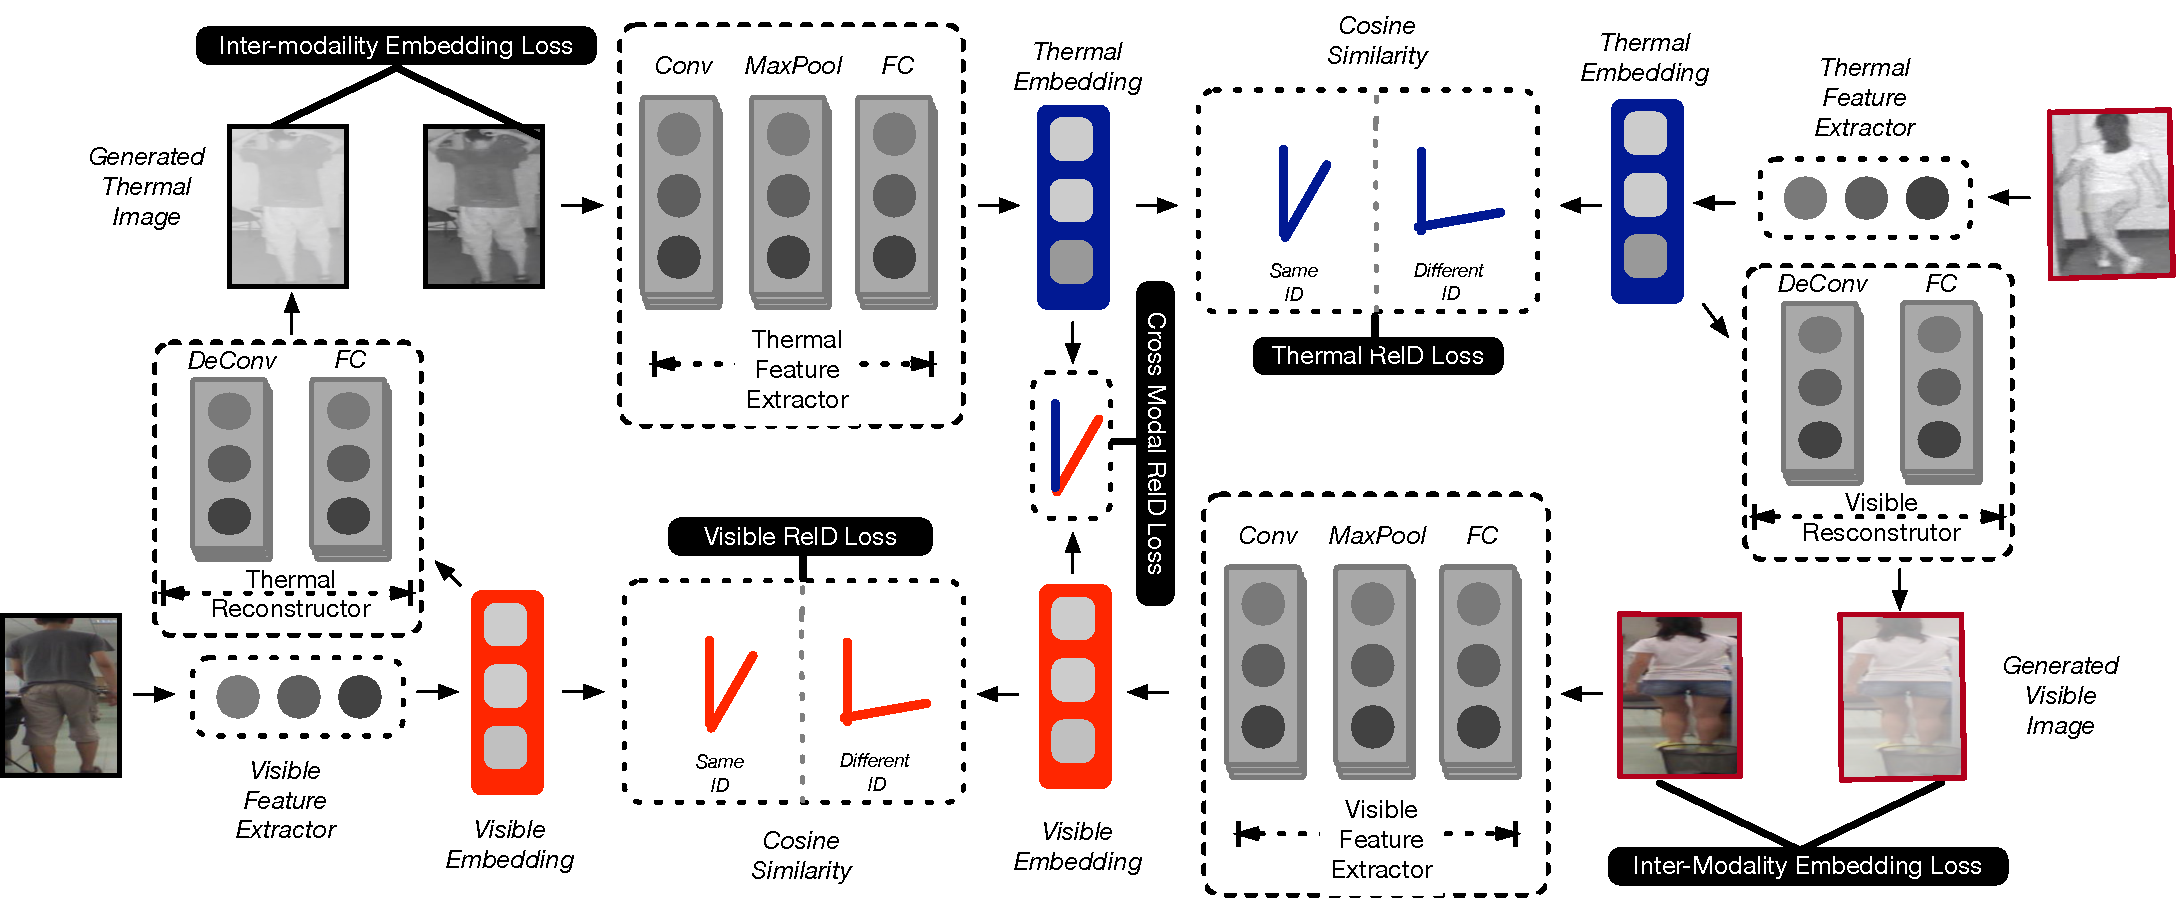
\includegraphics[width=15.0cm]{02/arch.pdf} \\
    \bicaption[跨模态行人重识别MAENet框架示意图]
      {本章提出的跨模态行人重识别MAENet框架的示意图。由图所示, Thermal特征提取器为一个卷积神经网络将从Thermal模态的图片提取特征向量。同样 Visible 特征提取器从Visible模态提取对应特征向量。对应Thermal 和 Visible 重建器从特征向量生成对应Thermal 和 Visible的图片。同时ReID loss是基于贝叶斯的成对损失函数用于跨模态和模态内检索训练。}
      {The framework of the proposed framework- MAENet in this chapter. As illustrated, the fhermal feature fxtractor is a convolutional neural network responsible for extracting feature vector from thermal images. in the same way, the visible feature extractor extracts features from the visible images. The thermal and visible reconstructors are responsible for reconstructing thermal and visible images. The reid losses are devised to perform cross-modal and intra-modal person re-identification.}   
      \label{fig:arch}
\end{figure} 
神经网络设计一个框架来提取对于模态和外表恒定的特征的想法。如图~\ref{fig:arch1}所示, 对于两个绿色框围住的两张来自同一行人的图片, 尽管他们的视觉图像特征截然不同, 但是两张图片中的行人展示出相似的轮廓特征, 这样的轮廓特征便可以帮助我们实现识别同一行人的任务。受这一发现的启发, 本章提出一个全新的框架图 \textbf{MAENet}, 用来完成跨模态的行人重识别任务。我们设计并且实现了一个新的模态和外表恒定编码的网络来提取由不同摄像头不同角度拍摄的同一行人照片的公共的特征。 如图~\ref{fig:arch} 所示, 框架类似于自编码器的架构, 由两个特征提取器 (Visible Feature Extractor 和 Thermal Feature Extractor) 以及两个图像重建器 (Thermal Reconstructor 和 Visible Reconstructor)组成。其中每个图像重建器会从同一行人的在同一模态的图像特征重建图片或者从另一模态的图片的特征重建当前模态的图片。例如, 对于来自同一行人$i$的图片$x_i$, $\hat{x}_i$, $y_i$ 其中 $x_i$ 和 $\hat{x}_i$是来在可见光模态的图片而$y_i$是来自于红外线模态的热度图片。我们的模型将从$x_i$提取的特征恢复成$y_i$图片, 并用L2损失来衡量恢复的优劣。同时也将从$x_i$的图片特征恢复成$\hat{x}_i$的图片, 从而促使模型学习到同一行人在不同的模态不同的外表下的共享的恒定的那一部分特征。
同时, 为了进行相似度学习, 我们设计了两种基于成对训练数据的损失函数来进行跨模态以及单模态的检索训练。本章的主要贡献可以概括为下面的三点:
\begin{enumerate}
    \item 本章提出了一个新型的模态和外表恒定特征编码的框架来提取跨模态和不同外表下的共享的那部分特征用于行人重识别任务。
    \item 本章设计并且推导了基于带权最大似然估计的损失函数用于保留跨模态的相似度以及进行模态内的相似度学习。据我们所知, 这是第一个基于最大似然估计推导应用于跨模态行人重识别的工作。
    \item 本章的算法在多个公共标准数据集上进行了完善的实验, 实验结果表明本章的算法比之前发表的工作具有更加优越的性能, 证实了提出的框架的有效性以及泛化性。
\end{enumerate}

\section{相关工作}
与本章所提出的算法相关的一些工作主要分为两个方面: ``行人重识别'' 和 ``跨模态行人重识别''。 接下来这一小节, 我们着重介绍这些方法的设计和实现以及我们的相关性。
\subsection{行人重识别}
和行人重识别相关的工作可以分成一下两个类别: ``基于手工特征的方法'' 和 ``基于深度学习的方法''。 \par
\textbf{基于手工特征的方法:} 
基于手工特征的核心方法是用人为去设计选取最具有分辨力的图像特征用于后阶段的度量学习~\cite{gray2008viewpoint, hu2013exploring, gheissari2006person, farenzena2010person, ma2012local, cheng2011custom}。Gray 和 Tao 提出~\cite{gray2008viewpoint}使用 AdaBoost 来动态的从色彩和纹理的特征中选取适用于检索的有判别性的特征。Farenzena 等人~\cite{farenzena2010person} 提出一种 Symmetry-Driven Accumulation of Local Features (SDALF)方法, 通过考虑对称性以及非对称性来处理行人图像的视角变化。Ma 等人~\cite{ma2012local} 将局部的描述符转换成 Fisher
Vector 来得到图片的一个全局的特征向量。 Cheng 等人~\cite{cheng2011custom} 基于Pictorial Structure 算法考虑分块的颜色信息来进行行人检索。Liao 等人随后提出了 Local Maximal Occurrence (LOMO), 通过分析纵向局部特征的出现频率, 并且通过最大化出现的频次来获得稳定的特征表示。 同时对于检索需要的度量学习, 通过跨视角的二次判别分析来学习一个子空间, 随后在子空间学习一个QDA的度量函数。LOMO 随后被~\cite{zhang2016learning} 以及~\cite{zhang2016sample} 采用来获取强健的图像表征。Chen~\cite{chen2015mirror} 提出一个基于零填充的特征变换策略来对齐不同视角的特征分布, 这种方法能极大提高现有模型的准确度。 Shi随后~\cite{shi2015transferring} 通过学习中等层次的语义特点例如发型, 鞋子款式 和着装等来获得更加有力的特征表示。 \par
\textbf{基于深度学习的方法:}
与基于手工特征方法不同的是, 基于深度学习的重识别方法使用深度神经网络根据监督信号自动提取图像
特征, 能得到更加有判别力强健的特征表示。基于深度学习的方法由于取得的优异的性能也已经成为了行人重识别的的主流方法。 \par
第一次将深度学习引入行人重识别任务的是~\cite{yi2014deep}和~\cite{li2014deepreid}。2014年, Dong~\cite{yi2014deep} 提出一个基于孪生卷积神经网络的架构直接从输入的图片提取特征, 然后基于二分类损失函数和反向传播优化神经网络。Wei~\cite{li2014deepreid} 等人提出 FPNN 使用一个统一的神经网络同时处理遮挡,背景繁杂等等行人重识别的难题, 并且使用负对数似然 (Negative Log Likelihood)损失函数进行成对的训练。随后, Lin 等人~\cite{wu2016personnet} 通过使用更小的卷积核加深了提取特征的卷积神经网络的深度, 极大的提高了重识别的准确度。Rahul Rama 等人~\cite{varior2016siamese} 将循环神经网络的一个经典架构-长短期记忆网络 (Long Short-term Memory, LSTM) 引入进重识别, 通过LSTM对图片的的分块特征进行序列化的建模来提高得到的图像特征的辨别能力。2018年, Sun 等人~\cite{sun2018beyond} 提出 PCB, 通过一个基于分块的卷积神经网络来提取细粒度的特征以及一个改进的分块池化策略 (RPP)来生成分块的特征向量, 最后通过在每个局部向量上进行分类损失计算来训练模型进行重识别检索任务。Feng~等人~\cite{feng2018learning} 提出在特征提取的阶段引入摄像视角的信息来减缓类内的变化带来的影响。Yu ~\cite{yu2019unsupervised} 探索了用无标签监督的方法进行行人重识别的可能性。Liu 等人~\cite{liu2019deep} 为了提高重识别算法在现实生活中的应用, 提出了使用human-in-the-loop的强化学习来收集数据不断的更新模型。 这样可以最大限度的减少人工标注数据的开销以及提高重识别模型的性能。随后, Eom 等人~\cite{eom2019learning}基于生成对抗网络提出 IS-GAN 用来对行人的表征解耦, 将行人的身份相关的特征从与身份无关的特征中解耦出来。尽管这些方法在许多的行人重识别数据集上获得了不错的性能表现, 他们都是专注解决单可见光模态的行人检索, 并不能直接被应用到跨模态的行人重识别任务中。
\subsection{跨模态行人重识别}
对于跨模态的行人重识别, 研究人员已经研究了 RGB-Depth~\cite{haque2016recurrent, munaro20143d, wu2017robust},  Text-Image ~\cite{li2017identity,li2017person,ye2015specific, yin2017adversarial}。本章研究的跨模态行人重识别主要指的Visible-Thermal 重识别 (VT-ReID)。 2017年, Wu 等人~\cite{wu2017rgb}第一次提出VT-ReID的概念, 并且提出了一个基于零填充的网络结构来学习公共的特征。2018年, Ye 等人~\cite{ye2018visible} 提出使用双流卷积神经网络来将两个模态的图片映射到可以比较的同一特征空间
\begin{figure}[!htp]
    \centering
    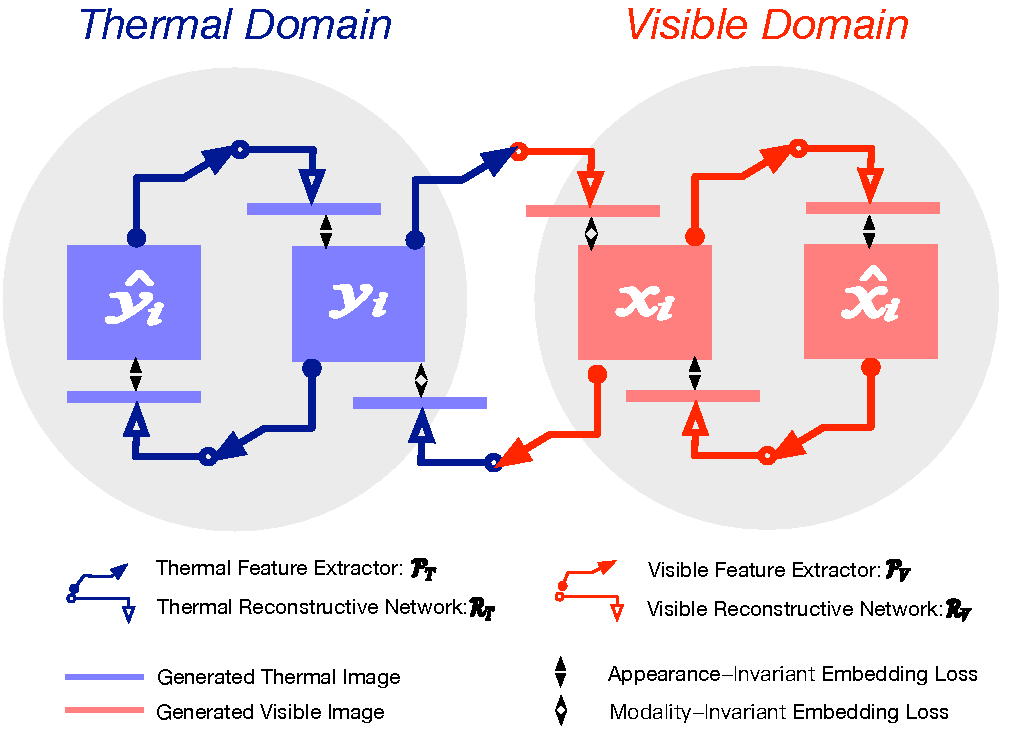
\includegraphics[width=12.0cm]{02/arch2.pdf} \\
    \bicaption[模态和外表恒定重建编码架构图]
      {模态和外表恒定重建编码的基础架构图。红色代表visible模态, 蓝色代表thermal模态。$x_i$ 和 $\hat{x}_i$是来自visible模态的同一行人图片, $y_i$和 $\hat{y}_i$是来自thermal模态的同一行人照片。由图所示, 使用了两种不同的损失函数来学习模态内外表恒定的特征以及跨模态恒定的特征。}
      {The illustration of modality and apperance invariant embedding framework. Red color represents the visible modality and blue color stands for the thermal modality. $x_i$ and $\hat{x}_i$ are person images from the visible modality while $y_i$ and $\hat{y}_i$ are from the thermal modality. Two embedding loss are enforced to learn  apperance-invariant and modality-invariant feature embeddings.}   
      \label{fig:arch2}
\end{figure} 

中。 同时基于排序损失, 作者提出了一个 Dual-Constrained Top-Ranking 的损失函数来减轻跨模态变化以及模态内变化带来的影响。随后, 作者改进了基础的双流神经网络, 在两个卷积神经网络后层的全连接网络共享权重。同时, 作者提出了一个二阶段学习策略, 第一阶段进行特征学习, 第二阶段进行度量学习, 通过一个分层次的跨模态匹配模型优化模态特有的以及模态共享的特征。2019年, Hao等人~\cite{hao2019dual} 基于 PCB 模型设计双流 PCB 主干结构, 在特征分布的层面对齐每一个分块的特征。随后, 他又提出一个新型的算法 HSME~\cite{hao2019hsme} 通过将特征映射到超球面, 然后在超球面进行特征嵌入学习。Ye 随后提出~\cite{ye2019modality}基于双流神经网络的模态感知的协同学习方法, 同时可以在特征层面以及分类器层面解决模态差异带来的影响。特征层面是通过双流神经网络来映射到相同的空间减轻模态差异的影响。在分类器层面则是通过两个模态特有的分类起来捕获模态特定的信息。然而, 前面提到的大多数的算法主要集中关注在后一阶段的度量学习来减轻模态差异以及模态内变化带来的影响, 忽略了在网络结构层面直接解耦提取出最适用于跨模态检索的有辨别性特征的重要性。

\section{MAENet}
\subsection{本章主要符号定义以及问题定义}
在整章中, 我们使用书法大写字母 (calligraphic uppercase), 例如 $\mathcal{X}$ 来表示映射函数。本章使用粗体大写字母 (Bold-face uppercase), 例如 $\mathbf{B}$ 来代表集合以及粗体小写字母来代表向量, 如 $\mathbf{b}$。 $U$代表向量空间。 \par
\textbf{问题定义:} 假设 $\mathbf{X}=\{k\}_{i=1}^N=\mathbf{V} \cup \mathbf{T}$ 是一个包含 $N$ 个训练样本的集合, 其中包含了来自visible 模态的行人照片$\mathbf{V}$以及thermal 模态的行人照片$\mathbf{T}$。$I_{k_i} = i$是一个特征函数将图片映射到它的索引。$\mathcal{S}: N * N \rightarrow\{0,1\}$是一个相似性映射函数。 $\mathcal{S}_{ij} = 1$ 如果 $k_i$ 和 $ k_j$ 图片是属于来自同一个人的照片。  $\mathcal{S}_{ij} = 0$ 如果 $k_i$ 和 $ k_j$ 图片是属于来自不同人的照片。 $\mathbf{P}=\left\{\left\{k_p, k_q: S_{p q}=1\right\}: p, q \in N\right\}$ 是一个包含了所有同一个行人图片对的集合。监督VT-ReID的目标就学习两个特征映射函数 $\mathcal{F}_V: \mathbf{V} \rightarrow \mathbf{U}$ 和 $\mathcal{F}_T: \mathbf{T} \rightarrow \mathbf{U}$, 其中需要满足: 给定任意的在检索图片集中的一张行人照片, 例如来自visible 模态的检索照片 $\mathbf{V}^{\prime} \subset \mathbf{V}$ 以及一个数据库 $\mathrm{T}^{\prime} \subset \mathrm{T}$, 找到 图片 $k \in \mathbf{T}^{\prime}$ 其中 $S_{I_v I_k}=1$。\par
本章提出一个基于深度学习的框架用于VT-ReID, 这个框架集成了增强的特征学习以及度量学习, 并且基于一种端到端的优化方法进行直接优化, 整个框架图如图~\ref{fig:arch}。
\subsection{混合双流特征提取架构}
混合双流特征提取架构如架构图~\ref{fig:arch}所示, 其包含两个模态特定的卷积神经网络$\mathcal{F}_V$ 和 $\mathcal{F}_T$ 来提取visible和thermal模态的图片特征。两个特征提取卷积神经网络的结构完全相同, 都是基于Resnet-50~\cite{he2016deep}。同时, 额外的全连接层添加在Resnet-50后来将特征映射到一个两个模态共享的特征空间。值得注意的是, 额外添加的两个全连接层共享参数, 以便于学习到模态共有的特征信息。
\subsection{模态和外表恒定的重建编码}
为了进一步保证上述从两个模态数据中提取的特征向量包括必要的有判别性的信息, 我们思考在特征层面增加额外的约束条件的可能性。受~\cite{cao2016correlation}使用基于自编码器的网络架构来提取跨模态关联的启发, 我们设计了一个新的网络结构如图~\ref{fig:arch2}所示。网络除了基础的双流卷积神经网络, 即thermal特征提取器$\mathcal{F}_T$和visible特征提取器$\mathcal{F}_V$之外, 还包含两个特征重建神经网络, 即thermal重建网络$\mathcal{R}_T$以及visible重建网络$\mathcal{R}_V$。为了生成模态恒定特征的损失函数可以由如下的公式表示: 
\begin{equation}
  L_{M I}=\sum_{\mathbf{Q} \in \mathbf{P}} \sum_{x_i, y_i \in \mathbf{Q}}\left(\left\|x_i-\mathcal{R}_V\left(\mathcal{F}_T\left(y_i\right)\right)\right\|_2^2+\left\|y_i-\mathcal{R}_T\left(\mathcal{F}_V\left(x_i\right)\right)\right\|_2^2\right).
  \label{eq:MI_loss}
\end{equation} 
其中$\mathcal{R}_V$和$\mathcal{R}_T$是基于反卷积的深度神经网络, 将特征向量重建成对应的visible模态的图片以及thermal模态的图片。$\mathcal{F}_V$和$\mathcal{F}_T$则是两个深度卷积神经网络从输入的图片提取特征并且映射成一个低维的特征向量。$x_i \in \mathbf{V}$ 是来自visible模态的图片, 而$y_i \in \mathbf{T}$是来自thermal模态的图片。同时, $x_i$ 和 $y_i$ 是来自同一行人$i$的两张属于不同模态的图片。通过降低此跨模态重建的误差$L_{M I}$, 从一个模态图片提取的特征向量则会学习到模态不变的特征以便于恢复成对应另一模态的图片。由于VT-ReID同时还受到模态内变化 (Intra-modality Variation) 的影响, 本章另外提出了一个外表恒定的损失函数来促使模型捕捉到在一个模态内同一行人在不同的摄像视角, 着装, 姿态等情况下的共享的信息, 如图~\ref{fig:arch2}右所示。外表恒定损失函数如下所示:
\begin{equation}
  \begin{aligned}
  L_{AI} = \sum_{\mathbf{Q} \in \mathbf{P}}\sum_{x_i,\hat{x_i},y_i,\hat{y_i} \in \mathbf{Q}}(&||x_i - \mathcal{R}_V(\mathcal{F}_V(\hat{x_i}))||_2^2+
      ||\hat{x_i} - \mathcal{R}_V(\mathcal{F}_V(x_i))||_2^2  \\
      +&||y_i - \mathcal{R}_T(\mathcal{F}_T(\hat{y_i}))||_2^2+ 
      ||\hat{y_i} -\mathcal{R}_T(\mathcal{F}_T(y_i))||_2^2).
  \end{aligned}
  \label{eq:AI_loss}
  \end{equation}
  其中$L_{A I}$表示两个模态的模态内外表恒定损失函数的集合, 其中$\hat{x}_i \in \mathbf{V}$ 且 $\hat{y}_i \in \mathbf{T}$ 是和$x_i$, $y_i$分别同模态同一个行人的不同照片。通过最小化损失函数$L_{A I}$, 特征提取器 $\mathcal{F}_T$或者$\mathcal{F}_V$会学习从同一个行人的不同照片中学习到对外观恒定的一部分特征, 例如行人的轮廓或者其他可以有助于识别定位的特征。我们将完整的重建损失定义为以上两种损失函数之和, 如下所示:
  \begin{equation}
    L_{RE} = L_{MI} +L_{AI}
    \label{eq:re}
\end{equation}
通过最小化~\ref{eq:re}这个损失函数, 特征学习神经网络$\mathcal{F}_T$和$\mathcal{F}_V$ 可以同时生成对模态和外观都不变的特征向量, 从而极大的提高后续检索任务的性能。
\subsubsection{基于成对关联的相似度学习}
为了有效的进行跨模态行人重识别任务, 以及支持单模态重识别的操作, 假设我们有两张来自于同一行人的照片$x_i$和$x_j$, 则它们两相对应的特征向量$\mathbf{x}_i$ 和 $\mathbf{x}_j$ 在特征空间上应该比较接近, 即有比较短的欧式距离, 反之亦然。为了更好的保证这一点, 我们设计了一个目标函数直接包含了三种损失函数: (1) 跨模态的成对检索损失函数 (2)模态内的成对检索损失函数 (3)分类损失函数。\par
假设, 我们有一个训练数据集$\mathbf{X}= \{x_i\}^B_{i=1}\cup\{y_j\}^B_{j=1}, B < N$, 我们可以通过对应的特征提取器$\mathcal{F}_T$ 和  $\mathcal{F}_V$得到对应的特征向量 $\mathbf{H} = \{h_i^V\}_{i=1}^B\cup\{h_j^T\}^B_{j=1}$, 其中 $h_i^V = \mathcal{F}_V(x_i)$ $x_i$是来自visible的图片。而对于来自thermal模态的图片$y_i$, 则有 $h_j^T = \mathcal{F}_T(y_j)$。相似性标签写作 $s^{mn}_{ij} = S_{I_{k_i^m}~I_{k_j^n}}$, 其中 $m$ 和 $n$代表模态。$I_{k^m_i}$表示第$i_{th}$章图片在模态$m$的数据集合中的索引。通常说来, $s^{VT}_{ij}=1$意味着第$i_{ith}$和第$j_{th}$组成的图片对 $(k^V_i,k^T_j)$ 分别来自visible和thermal模态, 并且它们属于同一个行人的不同照片。基于以上定义, 其似然函数可以正式描述为:
\begin{equation}
  p(s^{mn}_{ij}|h_i^m,h_j^n) = \sigma{(d(h_i^m,h_j^n))}^{s^{mn}_{ij}}(1 - \sigma{(d(h_i^m,h_j^n))})^{(1-s^{mn}_{ij})} \label{con:conditional} \\
\end{equation}
其中 $d(h_i^m,h_j^n) = \cos{(h_i^m,h_j^n)}$ 是 $h_i^m$和 $h_j^n$的余弦距离。同时, $\sigma(x) = \frac{1}{1+e^{-x}}$ 是sigmoid激活函数。 $ p(s^{mn}_{ij}|h_i^m,h_j^n)$表示在得到两个特征向量$h_i^m$ and $h_j^n$后 $s^{mn}_{ij}$ 的条件概率。同时, 我们另外定义了一个权重参数 $w_{ij}^{mn}$ 来解决数据不平衡的问题~\cite{cao2018deep}:
\begin{equation}
  w^{mn}_{ij} = 
  \begin{cases}
  |\mathbf{S}|/|\mathbf{S}^{mn}_1|, &s^{mn}_{ij}=1\\
  |\mathbf{S}|/|\mathbf{S}^{mn}_0|, &s^{mn}_{ij}=0 \\
  \end{cases}
\end{equation}
其中$\mathbf{S}^{mn}_1 = \{(i,j): s^{mn}_{ij}=1\}$是一个图片对的集合, 其中每个图片对都属于同一个行人。 $\mathbf{S}^{mn}_0 = \{(i,j): s^{mn}_{ij}=0\}$ 则是一个图片对的集合, 其中每个图片对包含的图片来自不同的行人。\par
接下来, 我们会展示跨模态行人重识别损失函数的推导过程。我们基于最大似然估计 (Maximum Likelihood Estimation, MLE) 来推导。用来进行跨模态检索的带权的最大似然估计的损失函数$L_{Inter}$ 如下式~\ref{eq:inter}所示:
\begin{equation}
  \begin{aligned}
     L_{Inter} &= -\log{ p(\mathbf{S}|\mathbf{H})} 
      =  -\sum_{i, j}w^{VT}_{ij}\log{p(s^{VT}_{ij}|h_i^V,h_j^T)} \\
      &= -\sum_{i,j}w^{VT}_{ij}(s^{VT}_{ij}d(h_i^V,h_j^T)-log(1+e^{d(h_i^V,h_j^T)}))
 \end{aligned}
 \label{eq:inter}
  \end{equation}
非常明显, 通过优化~\ref{eq:inter}, 相同图片对的余弦相似度会增加, 不同图片对的特征向量的余弦相似度会降低。但是由于$L_{Inter}$并没有考虑到单模态内的检索问题, 也没用考虑到模态内变化的影响, 因此, 自然我们需要针对visible模态和thermal模态设计两个模态内的重识别损失函数。\par
对于thermal模态的图片, 训练的图片对 $(y_i, y_j)$都是来自thermal模态的行人照片。和跨模态的重识别损失函数类比可得到模态内重识别损失函数的构造:
\begin{equation}
  L_{Intra\_Thermal} = -\sum_{i,j}w^{TT}_{ij}(s^{TT}_{ij}d(h_i^T,h_j^T)-log(1+e^{d(h_i^T,h_j^T)}))
  \label{eq:intrathermal}
\end{equation}
同样的, 我们也可以用相同的方式来推导出在visible模态的成对重识别损失函数:
\begin{equation}
  L_{Intra\_Visible} = -\sum_{i,j}w^{VV}_{ij}(s^{VV}_{ij}d(h_i^V,h_j^V)-log(1+e^{d(h_i^V,h_j^V)}))
  \label{eq:intravisible}
\end{equation}
这样, 模态内的重识别损失函数$L_{Intra}$则可视为visible和thermal的两个损失函数之和:
\begin{equation}
  L_{Intra} = L_{Intra\_Visible} + L_{Intra\_Thermal}
\label{eq:Intra}
\end{equation}
为了进一步提高学习到的表征的可辨别性, 如论文~\cite{ye2018visible}所示, 我们进一步继承了一个身份损失函数 (Identity Loss), 实际上也是一个分类损失函数, 将每一个行人当作一个类别, 并且使用softmax交叉熵来进行监督分类器的学习, 其可用正式的公式表示为:
\begin{equation}
  L_{\text {Identity}}=-\sum_{i=1}^N \log \frac{e^{\mathbf{W}_{y_i}^T \mathbf{h}_{\mathrm{i}}}}{\sum_{k=1}^C e^{\mathbf{W}_k^T \mathbf{h}_{\mathrm{i}}}}.
  \label{eq:identity}
\end{equation} 
其中 $\mathbf{W}_k$是对于第$k$个行人的权重向量, $N$是每个batch的图片数, 照片中的类别总数也就是行人的个数为$C$。值得注意的是, 我们分别对每个模态的特征进行分类学习。通过这种方式, 学习到的特征可以更多的保留与行人相关的特征, 也一定程度减轻了模态内变化的影响。\par
全面的训练目标函数可以视作上述所有的损失函数之和, 即:
\begin{equation}
  L_{total} = L_{Inter}+\lambda_1L_{Intra}+\lambda_2L_{Identity} + \lambda_3L_{RE}
\label{eq:total}
\end{equation}
其中, $\lambda_1$,~$\lambda_2$,~和 $\lambda_3$ 是三个预先设定好的系数用来控制各个不同损失函数在总体训练目标中的影响。
\subsection{优化算法}
本章的优化整个框架的算法如算法~\ref{algo:main}所示。我们有一个训练数据集$\mathbf{X}$ 以及对应的相似性标签$\mathbf{S}$。最初的学习率设置为$\alpha$, 并且我们分别设置三个超参数$\lambda_1, \lambda_2, \lambda_3$来平衡各个损失函数在公式~\ref{eq:total}中的影响。最大的迭代轮数设置为$T$。 首先, 我们将$\theta_{V}$和$\theta_{T}$用在ImageNet上预训练好的参数进行初始化。 然后, 我们基于Xavier初始化随机初始化$\theta_{RV}$和$\theta_{RT}$。迭代轮数计数器$t$被设置为 $0$。 \par
在模型未收敛并且迭代次数$t$比最大迭代次数$T$小时, 我们进行下列操作。首先, 我们将$t$增加$1$。然后, 根据采样策略从输入的数据集中$\mathbf{X}$随机采样一个batch的数据。将数据输入模型, 计算各个部分损失函数的数值。
随后, 计算梯度并且通过反向传播得到各个参数对应的梯度。最后根据梯度更新模型的参数。\par
以上操作循环进行直到模型收敛或者迭代次数超过设定的最大值。


\begin{algorithm}
  \caption{\textbf{MAENet}框架的优化算法}\label{algo:main}
  \KwData{训练图片集 $\mathbf{X}$,~相似性标签 $\mathcal{S}$, ~学习率 $\alpha$ and 损失函数系数 $\lambda_1$, $\lambda_2$, $\lambda_3$~ 最大迭代轮数$T$}
  \KwResult{优化的网络结构参数 $\theta_V$,~$\theta_T$, $\theta_{RV}$,~$\theta_{RT}$;}
  $t \leftarrow 0$\;
  $\theta_V \leftarrow ImageNet预训练参数$  \; 
  $\theta_T \leftarrow ImageNet预训练参数$  \; 
  $\theta_{RV} \leftarrow \textbf{Xavier}(\theta_{RV})$  \; 
  $\theta_{RT} \leftarrow \textbf{Xavier}(\theta_{RT})$  \; 
  \While{未收敛 \textbf{and} $t < T$}
  {
    $t \leftarrow t +1 $\;
   从 $\mathbf{X}$ 中采样 $Q_1, Q_2 \in \mathbf{P}, Q_1 \cap Q_2 = \emptyset $ 来得到$x_i$,~$\hat{x}_i$,~$y_i$,~$\hat{y}_i$ $\in  Q_1$, $x_j$,~$\hat{x_j}$,~${y_j}$,~$\hat{y_j} \in Q_2$ \;
   用 ~$\mathcal{F}_V(\bullet;\theta_V)$,~$\mathcal{F}_T(\bullet;\theta_T)$,~$\mathcal{R}_V(\bullet;\theta_{RV})$,~$\mathcal{R}_T(\bullet;\theta_{RT})$ 通过 Eq. \ref{eq:MI_loss}, \ref{eq:AI_loss}, \ref{eq:re} 计算 $L_{RE}$  \;
   对于 $p \in \{i, j\},~$,$h_p^V = \mathcal{F}_V(x_p;\theta_V)$, $h_p^T = \mathcal{F}_T(y_p;\theta_T)$ \;
   通过 Eq.~\ref{eq:Intra} 计算 $L_{Inter}$ \;
   通过 Eq.~\ref{eq:intrathermal} 计算 $L_{Intra\_Thermal}$ \;
   通过 Eq.~\ref{eq:intravisible} 计算 $L_{Intra\_Visible}$ \;
   通过 Eq.~\ref{eq:identity} 计算 $L_{Identity}$ \;
   $L_{total} \leftarrow L_{Inter} + \lambda_1 (L_{Intra\_Thermal} + Intra\_Visible) + \lambda_2 (L_{Identity}) + \lambda_3 (L_{RE}) $ \;
   反向传播得到 $\nabla_{\theta_*}$~$*\in \{V, T, RV, RT\}$ \;
  $\theta_* \leftarrow \alpha ( \theta_* - \nabla_{\theta_*}) $ \;
  }
 
  \end{algorithm}

\section{实验结果与分析}
本章进行了充足广泛的实验来验证我们提出的模型结构的有效性。在接下来的段落中, 本小节先介绍了数据集的设置以及基本信息, 然后阐述了本文使用的评估标准以及模型的实现细节。 随后, 本小节详细展示了本章提出的算法在各个标准数据集上取得的结果以及与先进的其他算法的比较细节来证明模型的性能。最后, 本小节展示了文章提出的消融实验来证明模型的各个组成部分的有效性。
\subsection{数据集}
本节的实验采取了两个标准的跨模态VT-ReID任务中数据集进行训练与测试。为了实现与现有的先进方法比较的公平公正, 我们采取标准的训练集和测试集的划分方法来进行对比实验。两个数据集的具体信息如下:
\begin{enumerate}
  \item \textbf{RegDB}~\cite{nguyen2017person} 是通过双摄像头系统的监控摄像机收集, 一共包含 $412$ 个行人。 对于每一个行人都包含十张来自visible模态的不同照片以及十张来自thermal模态的不同的照片。本小节采取~\cite{ye2018hierarchical}的实验方法, 将数据集随机分成两半, 一半组成训练集, 对应另一半是测试集。对于测试, 来自一个模态的所有图片当成检索图片, 对应另一个模态所有图片组成了被检索的数据库。 
  \item \textbf{SYSU-MM01}~\cite{wu2017rgb} 是一个由六个摄像机收集的大规模检索数据集, 包括4个可见光摄像头和2个红外摄像头。这个数据集由于包含室内和室外两种场景而显得更具有挑战性。 数据集一共包含$491$个行人, 每个行人至少包括两个摄像头拍摄的照片。 数据集标准测试有两个模式 \textit{indoor search} 和 \textit{all search}。对于 \textit{indoor search}模式, 即排除了在户外的摄像头拍摄的行人照片。由于 \textit{all search}显然更具有挑战性, 本节遵循 Ye et al ~\cite{ye2018visible} 主要采取 \textit{single-shot all search}的场景。 其中, 训练数据集包含$395$个行人, $22,258$ 张visible的图片以及$11,909$张thermal图片。 而测试数据集则包含$96$个行人, $3,803$张thermal的照片以及 $301$张visible的图片。在没有特殊说明的情况下, 均是使用thermal的图片进行检索, visible图片作为被检索的数据库。
\end{enumerate}
\subsection{评价指标}
我们采取平均准确率均值 (Mean Average precision, mAP) 以及累积匹配曲线 (Cumulative Matching Characteristic, CMC) 来评估方法的性能。其中 \textbf{mAP}的计算如下
\begin{equation}
   \textbf{mAP} = \frac{1}{n} \sum_{k=1}^{k= N} \textbf{AP}_k
\end{equation}
其中$N$是查询的图片总数。由此式可知, $mAP$则为每张图片的平均准确率的平均值。
\subsection{模型实现细节}
本章算法通过Pytorch 框架编码实现, 所有的实验是在一台4个Intel Core i7-4790K CPU核以及NVIDIA GeForce 1080Ti显卡上进行。全连接层后的输出维度设置为 2048, 两个数据集的 batch 大小设置为64。 Dropout率设置为 0.5。对于所有输入的图片, 首先会被缩放至 $256 \times 256$ 的大小, 随后会被随机裁剪成 $224 \times 224$的大小以便于输入进神经网络。在训练的阶段, 随机裁剪和随机水平反转被使用来进行数据增强以防止过拟合, 在测试阶段的话, 则使用中心裁剪。 超参数$\lambda_1$, $\lambda_2$和 $\lambda_3$均被设置成 $0.5$。本章采取 Momentum 优化器来进行优化神经网络, momentum设置为 $0.9$。 初使的学习速率设置为 $1e-3$。训练的最大轮数设置为$50000$。


\begin{table}[!htpb]
  %% \centering % not needed
  \bicaption{各个先进的算法在Visible到Thermal的跨模态重识别在\textbf{RegDB}数据集上的测试结果}{Vsible-to-Thermal Test Results of State of The Art Methods on RegDB}
  \centering
  \begin{tabular}{cccccc}
     \\ \hline 
  \multicolumn{2}{l|}{Methods} & r=1  &r=10 & r=20 & mAP   \\\hline
  
  \multicolumn{2}{l|}{HOG} & 13.49 & 33.22 & 43.66 & 10.31  \\
  \multicolumn{2}{l|}{MLBP} &  2.02& 7.33 & 10.90 & 6.77  \\
  \multicolumn{2}{l|}{LOMO\cite{liao2015person}} &  0.85& 2.47 & 4.10 & 2.28  \\
  \multicolumn{2}{l|}{GSM\cite{lin2016cross}} &  17.28& 34.47 & 45.26 & 15.06  \\

  \hline
  \hline
  \multicolumn{2}{l|}{SVDNet\cite{sun2017svdnet}} &  17.24& 34.12 & 44.51 & 19.04  \\
  \multicolumn{2}{l|}{PCB\cite{sun2018beyond}} & 18.32& 36.42 & 46.51& 20.13   \\ 
  \hline
  \hline
  \multicolumn{2}{l|}{TONE\cite{ye2018hierarchical}} &  16.87& 34.03 & 44.10 & 14.92  \\
  \multicolumn{2}{l|}{TONE + XQDA} &  21.94 & 45.05 & 55.73 & 21.80  \\
  \multicolumn{2}{l|}{TONE + MLAPG} &  17.82 & 40.29 & 49.73 & 18.03  \\
  \multicolumn{2}{l|}{TONE + SCDL} &  8.06 & 22.09 & 28.89 & 10.03  \\
  \multicolumn{2}{l|}{TONE + rCDL} &  9.47 & 22.96 & 29.42 & 10.26  \\
  \multicolumn{2}{l|}{TONE+HCML }& 24.44 & 47.53 & 56.78 & 20.80 \\
  \multicolumn{2}{l|}{Zero-Padding\cite{wu2017rgb} }& 17.75 &34.21 & 44.35 & 18.90  \\
  \multicolumn{2}{l|}{cmGAN\cite{dai2018cross} }& - & - & - & -  \\
  \multicolumn{2}{l|}{BDTR (ResNet50)\cite{ye2018visible} }& \textcolor{blue}{30.56} & \textcolor{blue}{54.62} & \textcolor{blue}{65.42} & \textcolor{blue}{32.45}  \\
  \hline
  \hline
   \multicolumn{2}{l|}{\textcolor{red}{MAENet} (ResNet50) }&\textcolor{red}{\textbf{44.32}} & \textcolor{red}{\textbf{63.98}} & \textcolor{red}{\textbf{72.67}} & \textcolor{red}{\textbf{45.55}} \\
   \hline
   \hline
  \end{tabular}
  \label{table:visiblethermalRegdb}
\end{table}
\subsection{与其他先进的方法在标准数据集上的结果比较}
我们与解决VT-ReID的先进算法模型在标准数据集上进行性能。具体地, 我们包括了几种基于深度学习的最先进的模型进行仔细的分析研究: \textbf{TONE+HCML}~\cite{ye2018hierarchical}, \textbf{cmGAN}~\cite{dai2018cross}, \textbf{Zero-Padding}~\cite{wu2017rgb}和 \textbf{BDTR}~\cite{ye2019bi}。我们也包括了几种其他的方法, 大部分其他算法的性能来自于~\cite{ye2019bi}。 选择进行比较的算法可以主要分成两类: 基于特征提取的方法 (\textbf{HOG}, \textbf{MLBP}, \textbf{LOMO}~\cite{liao2015person}), 基于匹配模型的方法 (\textbf{XQDA}, \textbf{GSM}~\cite{lin2016cross}, , \textbf{SCDL}~\cite{wang2012semi}, \textbf{rCDL}~\cite{huang2013coupled}, \textbf{MLAPG}~\cite{liao2015efficient})。我们额外加入两个在单模态行人重识别上的先进算法 \textbf{SVDNet}~\cite{sun2017svdnet} 和 \textbf{PCB}~\cite{sun2018beyond} 进行比较。\par
如表格~\ref{table:visiblethermalRegdb} 以及表格~\ref{table:visiblethermalsysu}所示, 本章提出的模型\textbf{MAENet}在 \textbf{RegDB} 和 \textbf{SYSU-MM01}数据集上与现有的先进算法相比较均取得了较大的性能提升。 很明显, 在\textbf{RegDB} 数据集上, 本章的算法比第二先进的算法\textbf{BDTR}在提高了 $13.1 \%$
的\textbf{mAP}, 在$Rank-1$准确度上提高了接近$13.8$。 而在~\textbf{SYSU-MM01} 数据集上 \textit{single-shot all search}场景下, \textbf{MAENet} 也取得了非常优秀的性能表现, 比\textbf{BDTR}提高了 $13.25 \%$ \textbf{mAP}。

\begin{table}[!htpb]
  %% \centering % not needed
  \bicaption{各个先进的算法在Visible到Thermal的跨模态重识别在\textbf{SYSU-MM01}数据集上的测试结果}{Vsible-to-Thermal Test Results of State of The Art Methods on SYSU-MM01}
  \centering
  \begin{tabular}{cccccc}
     \\ \hline
  \multicolumn{2}{l|}{Methods} & r=1 &r=10 & r=20 & mAP   \\\hline
  
  \multicolumn{2}{l|}{HOG} & 2.77 & 18.24 & 31.91 & 4.24  \\
  \multicolumn{2}{l|}{MLBP} & 2.12 & 16.23 & 28.32 & 3.86  \\
  \multicolumn{2}{l|}{LOMO\cite{liao2015person}} &  1.75 & 14.14 & 26.63 & 3.48 \\
  \multicolumn{2}{l|}{GSM\cite{lin2016cross}} &  5.29 & 33.71 & 52.95 & 8.00  \\

  \hline
  \hline
  \multicolumn{2}{l|}{SVDNet\cite{sun2017svdnet}} & 14.64 & 53.28 & 64.24 & 15.17  \\
  \multicolumn{2}{l|}{PCB\cite{sun2018beyond}} & 16.43 & 54.06 & 65.24 & 16.26  \\ 
  \hline
  \hline
  \multicolumn{2}{l|}{TONE\cite{ye2018hierarchical}} &  12.52 & 50.72 & 68.60 & 14.42  \\
  \multicolumn{2}{l|}{TONE + XQDA} &  14.01 & 52.78 & 69.06 & 15.97  \\
  \multicolumn{2}{l|}{TONE + MLAPG} &  12.43 & 50.64 & 68.72 & 14.61  \\
  \multicolumn{2}{l|}{TONE + SCDL} &  6.58 & 35.62 & 56.32 & 10.32  \\
  \multicolumn{2}{l|}{TONE + rCDL} &  7.02 & 37.31 & 57.64 & 10.46  \\
  \multicolumn{2}{l|}{TONE+HCML }& 14.32 & 53.16 & 69.17 & 16.16 \\
  \multicolumn{2}{l|}{Zero-Padding\cite{wu2017rgb} }& 14.80 & 54.12 & 71.33 & 15.95  \\
  \multicolumn{2}{l|}{cmGAN\cite{dai2018cross} }& 26.97 & 67.51 & 80.56 & 27.80  \\
  \multicolumn{2}{l|}{BDTR (ResNet50)\cite{ye2018visible} }& \textcolor{blue}{20.84} & \textcolor{blue}{63.81} & \textcolor{blue}{79.14} & \textcolor{blue}{22.86}  \\
  \hline
  \hline
   \multicolumn{2}{l|}{\textcolor{red}{MAENet} (ResNet50) }&\textcolor{red}{\textbf{29.79}} & \textcolor{red}{\textbf{77.24}} & \textcolor{red}{\textbf{89.87}} & \textcolor{red}{\textbf{36.11}} \\
   \hline
   \hline
  \end{tabular}
  \label{table:visiblethermalsysu}
\end{table}
在 $Rank-1$准确度上也提高了 $8.95 \%$。 同时由表~\ref{table:visiblethermalRegdb}和表~\ref{table:visiblethermalsysu}可知, 传统的单模态的行人重识别算法例如\textbf{PCB} 和 \textbf{SVDNet}并不能取得令人满意的结果, 尽管这两个算法在单模态检索的数据集上表现优异。主要原因是单模态的行人重识别算法没有考虑进来两个不同模态的差异 (Modality Discrepancy), 并不能充足的对齐两个不同模态的特征。而我们的方法由于采取了双流的神经网络进行特征提取, 并且通过多个基于贝叶斯的损失函数来进行特征对齐, 可以有效的减少模态差异带来的影响。同时, 和非深度学习的方法例如 ~\textbf{HOG} 和 ~\textbf{GSM} 等相比较时, 我们的方法更是一个明显的赢家。在 \textbf{RegDB}数据集上, 取得最佳效果的非深度学习方法时~\textbf{GSM}, 得到 $15.06 \%$ \textbf{mAP}。而在 \textbf{SYSU-MM01} 上, ~\textbf{GSM}获得$8.00$ ~\textbf{mAP}。 比本章提出的算法效果分别低 $30.5 \%$ 和 $28.11 \%$。导致基于非深度学习的算法性能不足的主要原因是基于传统手工方法提取的难以保留行人图像中的具有辨别力的特征。同时, 和其他基于深度学习的VT-ReID 方法例如~\textbf{TONE-HCML}, \textbf{cmGAN}, \textbf{Zero-Padding}相比较, 本章的算法也在各个评估指标上显著超出这些方法。

\begin{table}[!htpb]
  %% \centering % not needed
  \bicaption{各个先进的算法在Visible到Thermal的跨模态重识别在\textbf{SYSU-MM01} (Indoor)数据集上的测试结果}{Vsible-to-Thermal Test Results of State of The Art Methods on SYSU-MM01 (Indoor)}
  \centering
  \begin{tabular}{cccccc}
     \\ \hline
  \multicolumn{2}{l|}{Methods} & r=1 &r=10 & r=20 & mAP   \\\hline
  
  \multicolumn{2}{l|}{HOG} & 3.22 & 24.68 & 44.52 & 7.25  \\
  \multicolumn{2}{l|}{MLBP} & 3.43 & 26.42 & 45.36 & 7.72  \\
  \multicolumn{2}{l|}{LOMO\cite{liao2015person}} &  2.24 & 22.53 & 41.53 & 6.64 \\
  \multicolumn{2}{l|}{GSM\cite{lin2016cross}} &  9.46 & 48.98 & 72.06 & 15.57  \\

  \hline
  \hline
  \multicolumn{2}{l|}{SVDNet\cite{sun2017svdnet}} & 20.24 & 64.32 & 83.62 & 28.74  \\
  \multicolumn{2}{l|}{PCB\cite{sun2018beyond}} & 22.63 & 65.24 & 83.92 & 30.46  \\ 
  \hline
  \hline
  \multicolumn{2}{l|}{TONE\cite{ye2018hierarchical}} &  20.82 & 68.86 & 84.46 & 26.38  \\
  \multicolumn{2}{l|}{Zero-Padding\cite{wu2017rgb} }& 20.58 & 68.38 & 85.79 & 26.92  \\
  \multicolumn{2}{l|}{cmGAN\cite{dai2018cross} }& 31.63 & 77.23 & 89.18 & 42.19  \\
  \multicolumn{2}{l|}{BDTR (ResNet50)\cite{ye2018visible} }& \textcolor{blue}{31.92} & \textcolor{blue}{77.18} & \textcolor{blue}{89.28} & \textcolor{blue}{41.86}  \\
  \hline
  \hline
   \multicolumn{2}{l|}{\textcolor{red}{MAENet} (ResNet50) }&\textcolor{red}{\textbf{38.54}} & \textcolor{red}{\textbf{86.10}} & \textcolor{red}{\textbf{95.61}} & \textcolor{red}{\textbf{49.68}} \\
   \hline
   \hline
  \end{tabular}
  \label{table:sysuindoor}
\end{table}
同时, 我们也在 \textbf{SYSU-MM01} (single-shot indoor search)模式下进行了实验。 室内模式的场景排除了在室外的摄像头所拍摄的所有的行人照片。 首先, 由表~\ref{table:sysuindoor}所示, 本章提出的框架~\textbf{MAENet}在各个评价指标上均显著超越所有比较的方法。 \textbf{MAENet} 获得了$49.68 \%$ \textbf{mAP} 和 $38.54 \%$ $Rank-1$准确度, 比第二高的评估结果分别高出$7.5$和$6.6$个百分点。 同时, 和表~\ref{table:visiblethermalRegdb}和~\ref{table:visiblethermalsysu}相似, 单模态的重识别算法 ~\textbf{SVDNet}和~\textbf{PCB}取得的结果仍然不理想。同时, 基于非深度学习的方法依然不能得到令人满意的性能。但是相比较在(single-short all search) 场景下, 所有算法均取得了比较大的性能提升。 例如, 相比较而言, ~\textbf{GSM} 取得了 $15.57 \%$ ~\textbf{mAP}, 提升了 $7.57 \%$。单模态的行人重识别算法如~\textbf{PCB}的性能提升更为显著, 获得了 $14.2 \%$的性能提升。本章的算法 ~\textbf{MAENet} 也在\textbf{mAP}上提升了 $13.57$个百分点。 这些性能的提升是由于 (indoor search) 场景排除了室外的照片, 因此模态内的变化显著降低, 从而也极大的降低了重识别的难度。
\subsection{消融实验结果分析}
在这一小节, 我们仔细并且彻底的分析本章提出的框架中各个部分的损失函数对整个模型性能的影响。我们分别设计了几个变种模型如下所示:


\begin{figure}[!htp]
  \centering
  \begin{subfigure}{0.45\textwidth}
    \centering
    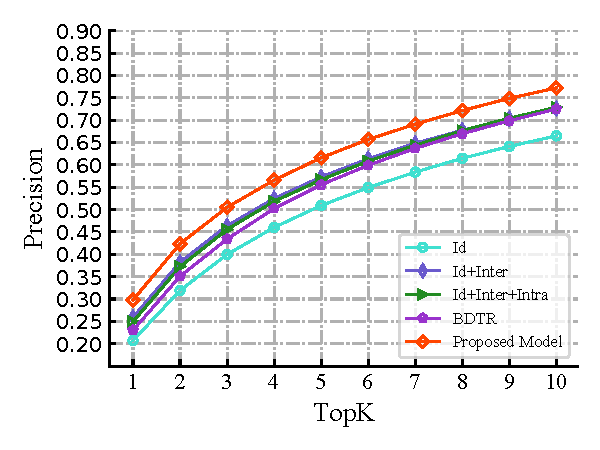
\includegraphics[height=5cm]{02/v_t_sysu_all.pdf}
    \caption{在SYSU-MM01 (All setting)下从visible模态到thermal模态的重识别结果}
  \end{subfigure}
  \hspace{1cm}
  \begin{subfigure}{0.45\textwidth}
    \centering
    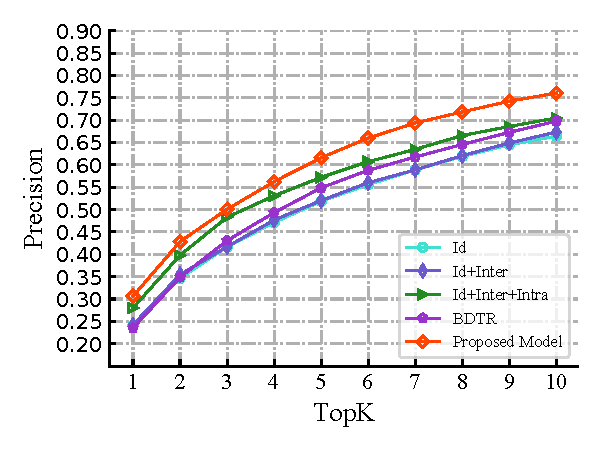
\includegraphics[height=5cm]{02/t_v_sysu_all.pdf}
    \caption{在SYSU-MM01 (All setting)下从thermal模态到visible模态的重识别结果}
  \end{subfigure}
  \begin{subfigure}{0.45\textwidth}
    \centering
    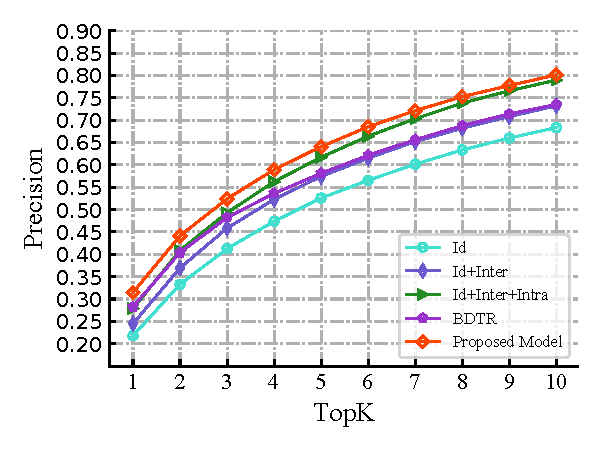
\includegraphics[height=5cm]{02/v_t_sysu_indoor.pdf}
    \caption{在SYSU-MM01 (Indoor setting)下从visible模态到thermal模态的重识别结果}
  \end{subfigure}
  \hspace{1cm}
  \begin{subfigure}{0.45\textwidth}
    \centering
    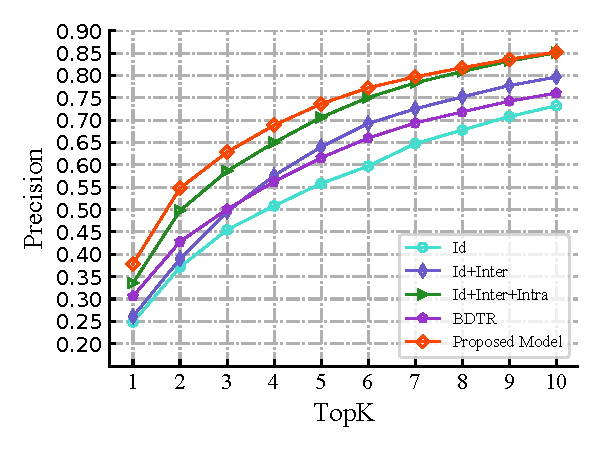
\includegraphics[height=5cm]{02/t_v_sysu_indoor.pdf}
    \caption{在SYSU-MM01 (Indoor setting)下从thermal模态到visible模态的重识别结果}
  \end{subfigure}
  \begin{subfigure}{0.45\textwidth}
    \centering
    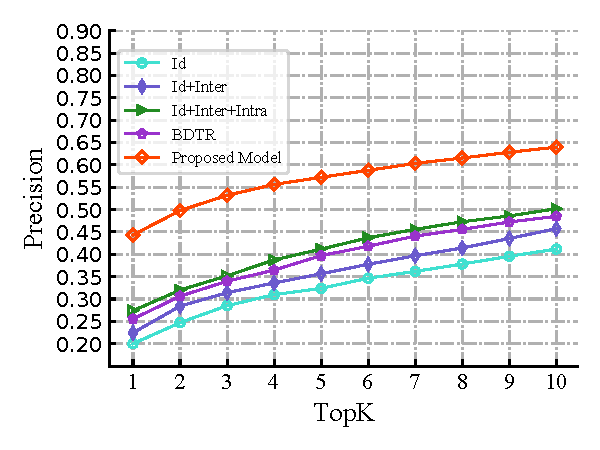
\includegraphics[height=5cm]{02/v_t_regdb.pdf}
    \caption{在RegDB下从visible模态到thermal模态的重识别结果}
  \end{subfigure}
  \hspace{1cm}
  \begin{subfigure}{0.45\textwidth}
    \centering
    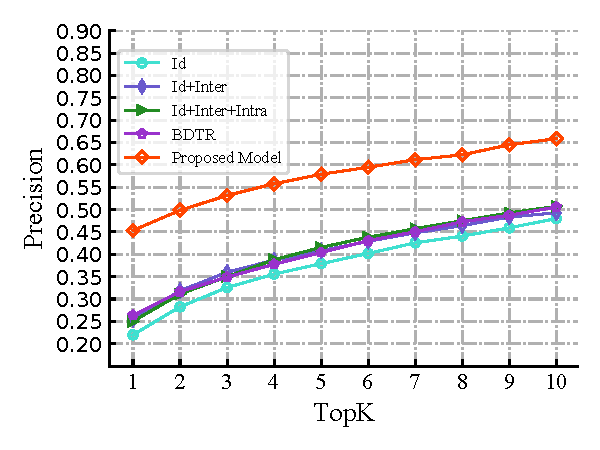
\includegraphics[height=5cm]{02/t_v_regdb.pdf}
    \caption{在RegDB下从thermal模态到visible模态的重识别结果}
  \end{subfigure}
  \bicaption[在两个不同数据集下的消融实验结果]{在两个数据集下模型的不同变种的行人重识别结果}{The person re-identification results of different variants on two public benchmark datasets.}
  \label{fig:ablation_res}
\end{figure}


\begin{enumerate}
  \item \textbf{Id}: 仅仅包含身份分类的损失函数$L_{Identity}$
  \item \textbf{Id + Inter}: 仅包含跨模态重识别损失函数$L_{Inter}$以及基于身份的分类损失函数$L_{Id} $的模型。
  \item \textbf{Id + Inter + Intra}: 不包含重建编码损失函数$L_{RE}$的模型。
  \item \textbf{BDTR}: 当时的基于双流神经网络的最先进模型。 由于我们的方法也是基于相同双流神经网络, 我们将BDTR也加入到消融实验进行对比研究。
  \item \textbf{Proposed Model}: 即本章提出的完整模型 \textbf{MAENet}
\end{enumerate}

由图~\ref{fig:ablation_res}可知, 仅包含分类损失函数的模型 \textbf{Id} 在~\textbf{SYSU-MM01} 和 \textbf{RegDB}上的所有测试场景均只能取得最低的性能。这是由于 \textbf{Id} 并不能有效的降低类内变化以及跨模态变化带来的影响。当加上 $L_{Inter}$损失函数后, 如图中的蓝色曲线所示, 模型在各个场景下都取得了性能上的提升。这是由于 $L_{Inter}$可以较大的对齐两个模态的特征, 降低跨模态差异带来的负面影响。同时当进一步加上$L_{Intra}$时, 如绿色曲线所示, 模型的性能进一步提升, 甚至可以显著的超越 \textbf{BDTR} 的性能。最终, 当我们加上本章提出的创新性的模态以及外表恒定的模块时候, 如红色曲线所示, 我们可以看到性能的显著提升。在 visible-to-thermal重识别场景, 这个模块在 \textbf{RegDB} 和 \textbf{SYSU-MM01} (all search)数据集上, 将$Rank1$准确率从$27.28 \%$, $24.93 \%$ 分别提升到了$44.32\%$ $32.33 \%$。在 thermal-to-visible的重识别场景中, 也可以观察到类似的性能提升。在 \textbf{RegDB}中$Rank1$ 准确度从 $25.00 \%$ 提升到了 $45.34 \%$ 而在 \textbf{SYSU-MM01} (indoor search) 从 $33.56 \%$ 提升到了 $37.86 \%$。这些显著的性能提升是由于我们提出的模态恒定以及外观恒定的网络以及损失函数可以帮助有效的对齐两个模态的特征, 降低模态间的差异, 降低跨模态变化以及模态内同一行人的不同变化带来的影响, 证实了这些不同的模块的有效性。

\section{总结}
本章针对图像检索的一个经典的应用行人重识别进行了深入的研究。本章针对行人重识别问题的一个非常具有挑战性的子问题-"跨模态行人重识别"进行了建模。 我们提出了一个崭新的神经网络框架以及对应的优化损失函数来进行学习。为了应对跨模态行人重识别的模态差异的带来的影响(Modality Discrepancy), 本章采取双流卷积神经网络分别将visible和thermal模态的照片映射到可比较的特征空间。同时, 基于autoencoder, 我们提出了一个模态和外表恒定的自编码网络架构 (modality and apperance invariant reconstructive embedding) 来提取出对于模态和外表都不变的特征。 为了进行重识别任务, 本章基于最大似然估计提出两种基于成对图片的重识别损失函数来进一步对齐两个模态的特征, 以及应对跨模态(Inter-modality Variation)和模态内的变化 (Intra-modality Variation)。